\documentclass[12pt]{memoir}

\def\nsemestre {V}
\def\nterm {Verano}
\def\nyear {2021}
\def\nprofesor {Adri\'an Barquero y Dar\'io Mena}
\def\nsigla {MA0609}
\def\nsiglahead {T\'opicos en Teor\'ia de N\'umeros}
\def\darktheme {}
\input{headerVarillyDiff}

\begin{document}
%\clearpage
\maketitle
%\thispagestyle{empty}
{\small
\setlength{\parindent}{0em}
\setlength{\parskip}{1em}

La teoría de curvas elípticas tiene al día de hoy más de 50 años de ser desarrollada continuamente. Fermat estudió ecuaciones que tenían relación  con curvas elípticas y es hasta el día de hoy que se pueden ver las relaciones con estos temas. Este tema se puede ver desde las distintas areas de la matemática: análisis, álgebra, geometría... Hay métodos para el uso de firmas digitales y seguridad en tarjetas de crédito que están relacionados con curvas elípticas.\par
En fín, este tema es de mucho interés en la actualidad. Nosotros nos centraremos en los números racionales siguiendo la línea del libro de Silverman \& Tate \cite{SilvermanTate}. En concreto los temas a tratar son los siguientes:
\begin{enumerate}
  \item Introducción a geometría proyectiva.
  \item Curvas cúbicas y ecuaciones en forma normal de Weierstrass.
  \item Suma de puntos y la ley de grupo en curvas elípticas.
  \item Puntos de orden finito y el teorema Nagell-Lutz.
  \item La estructura del grupo de puntos racionales en una curva elíptica y el teorema Mordell-Weil.
\end{enumerate}


\subsubsection*{Requisitos}
Se asume un conocimiento básico de teoría de números. Se utilizarán conceptos de teoría de grupos y variable compleja a un nivel básico.
}
\newpage
\tableofcontents
%\begin{multicols}{2}

\chapter{Curvas elípticas}

\section{Día 1| 20210105}

\subsection{Introducción a la geometría proyectiva}

\subsubsection{La vista algebraica}

En general hay más de una manera en la que uno puede construir el plano proyectivo y más generalmente el espacio proyectivo en varias dimensiones. A manera de motivación, a la hora de estudiar ciertos problemas en matemática, se llega a observar que es suficiente trabajar con objetos en términos de clases de equivalencia.\par
Por ejemplo un problema que se discute en el Silverman y Tate \cite{SilvermanTate}, al estudiar las soluciones racionales de la ecuación
$$x^N+y^N=1,$$
se puede ver que si $x=\frac ac$ y $y=\frac bd$ son soluciones racionales en su forma más reducida ($\mcd(a,c)=\mcd(b,d)=1$, y $c,d>0$) entonces debe ocurrir que $c=d$. Esto se logra después de un breve análisis de divisibilidad. Concluimos que la solución debe tener la forma $x=\frac ac$ y $y=\frac bc$.\par
Esta solución satisface que $a^N+b^N=c^N$ por lo que la solución $\left(\frac ac,\frac bc\right)$ del problema en términos racionales genera una solución $(a,b,c)$ de la ecuación homogénea $x^N+y^N=z^N$. La clave aquí es que como la ecuación es homogénea, cualquier múltiplo de $(a,b,c)$, $(ta,tb,tc)$ con $t\in\bR$, va a ser una solución al mismo problema. Pero como estas soluciones se obtienen de manera relativamente trivial, podríamos querer considerarlas como equivalentes. Este tipo de razonamiento lleva a la definición algebraica del plano proyectivo.

\begin{Def}
  El \term{plano proyectivo} sobre un cuerpo $K$ es el cociente del conjunto $\set{(a,b,c)\in K^3\less\set{(0,0,0)}}$ por la relación
  $$(a,b,c)\sim (a',b',c')\iff \exists t\in K^\x(a=ta',\ b=tb', c=tc').$$
  Denotamos entonces
  $$\bP^2_K=\quot{\set{x\in K^3\less\set{0}}}{\sim},$$
  y la clase de equivalencia de $(a,b,c)$ la denotamos $[a,b,c]$ y se llamarán sus coordenadas homogéneas.
\end{Def}

\begin{significant}
  ¿Qué pasa si incluimos el cero en nuestra definición del plano proyectivo?
\end{significant}

Bueno, volviendo al ejemplo que presentamos, nos gustaría que nuestras soluciones estén en correspondencia. Claramente $(0,0,0)$ resuelve la ecuación homogénea, pero no la que tiene forma racional. Quizás de manera más interesante, $(1,-1,0)$ resuelve la ecuación homogénea con exponente impar. Pero esta no da una solución de la ecuación racional, entonces podríamos pensar por ejemplo que tenemos $((a_j,b_j,c_j))\subseteq\bR^3$ una sucesión de soluciones reales que converge a $(1,-1,0)$ y $c_j>0$. Esta sucesión si genera soluciones $\left(\frac{a_j}{c_j},\frac{b_j}{c_j}\right)$ de la ecuación racional y cuando $j\to\infty$ entonces este par ordenado tiende a $(\infty,-\infty)$. Podemos entonces pensar que las tripletas con tercera coordenada nula corresponden con soluciones que se encuentran en el infinito. Esta clase de puntos en el infinito es fundamental y lo estudiaremos más adelante.

\begin{Def}
  El \term{espacio proyectivo} en $n$ dimensiones sobre un cuerpo $K$ es el conjunto
  $$\bP^n_K=\quot{\set{x\in K^{n+1}\less\set{0}}}{\sim}$$
  donde la equivalencia es $x\sim x'\iff \exists t\in K^\x(x=tx')$. De igual manera denotamos la clase de $x$ como $[x]$. Las coordenadas de $[x]$ igualmente se llamarán \term{coordenadas homogéneas}.
\end{Def}

Más adelante vamos a definir curvas en el espacio proyectivo. En este momento vamos a definir lo que entenderemos como una recta en el plano proyectivo. En principio verificar que un punto proyectivo $[a,b,c]$ está en una recta proyectiva consiste en ver que cualquier elemento de la clase de equivalencia satisface la ecuación mencionada.

\begin{Def}[Recta en el plano proyectivo]
  Una recta en el plano proyectivo $\bP^2_K$ es el conjunto de puntos $[a,b,c]$ cuyas coordenadas satisfacen una ecuación de la forma
  $$\al X+\bt Y+\ga Z=0,$$
  donde $\al,\bt,\ga\in K$ no son todos nulos.
\end{Def}

En en el plano usual, una recta es el conjunto de puntos que satisface una ecuación $\al x+\bt y+\ga=0$. En el caso proyectivo, la definición de recta que obtuvimos es básicamente lo que obtendríamos de esta ecuación al hacerla homogénea.

\subsubsection{Una visión geométrica}

Sabemos que en $\bR^2$ vale que dos puntos determinan una única recta y similarmente dos rectas se intersecan en un único punto salvo cuando son paralelas. Entonces buscamos extender el concepto de obtener una noción más completa, ¡quisiéramos poder decir que cualesquiera dos rectas se intersecan en un punto!\par 
La idea va a ser asociar a cada recta en el plano una \emph{dirección}. Al hacer esto, estaríamos agregándole un poco más de \emph{información} a una recta. Entonces una recta va a ser el conjunto de puntos \emph{y una dirección}. Para nosotros, dos rectas paralelas tendrán la misma dirección y como decimos ahora que la dirección es parte de la recta, las paralelas \emph{coinciden en la intersección}.\par 
Extendemos el concepto de recta agregando ``la dirección'' como un punto. Si trabajamos sobre $\bR$, habrá que agregar un número infinito de puntos. Porque si agregamos sólo un punto en el infinito como dirección entonces dos pares de rectas paralelas se intersecan en el mismo punto. En particular dos rectas distintas se intersecarían en dos puntos y eso contradice el hecho de que dos rectas distintas se intersecan en un único punto. Esto nos lleva a una idea geométrica para definir el plano proyectivo. 

\begin{Def}[Plano afín sobre $K$]
  Sea $K$ un cuerpo, el \term{plano afín} sobre $K$ es el conjunto $\bA^2_K=\set{(x,y)\in K^2}$. 
\end{Def}

\begin{Def}[Espacio afín n-dimensional]
  El \term{espacio afín} sobre un cuerpo $K$ es el conjunto $\bA^n_K=\set{(x_1,x_2,\dots,x_n)\in K^n}$. 
\end{Def}

Observe ahora la diferencia aquí con el plano proyectivo, se necesitaban tres coordenadas. Aquí en el plano afín necesitamos sólo dos. Análogamente en el espacio proyectivo de $n$ dimensiones, necesitamos $n+1$ coordenadas, mientras que en el $n$-espacio afín usamos $n$ coordenadas.

\begin{Def}[Plano proyectivo sobre K (geometricamente)]
  El \term{plano proyectivo} se define como el conjunto 
  $$\bP_K^2=\bA_K^2\cup\set{\text{direcciones en }\bA_K^2}.$$
  Consideramos que dos rectas en $\bA_K^2$ tienen la misma dirección cuando son paralelas.
\end{Def}

Por tanto una dirección se puede considerar como una clase de equivalencia de rectas. Definimos una equivalencia en el conjunto de las rectas en $\bA_K^2$ al considerar dos rectas como equivalentes cuando son paralelas. Así las direcciones en $\bA^2_K$ son las clases de equivalencia de rectas paralelas.\par 
Entonces los puntos de $\bP_K^2$ correspondientes a las direcciones, los llamamos ``puntos en el infinito''. Al conjunto de puntos en el infinito de hecho lo consideramos una recta en $\bP_K^2$, se le llama \term{recta en el infinito}. 
\begin{Ex}
  La noción de punto en el infinito se puede asociar con la idea de ver un par de lineas de tren. Desde un punto de vista, cuando se ve en la dirección de las lineas en una situación adecuada, pareciera que en el horizonte las lineas se tocan.\par 
  \red{TO DO: Agregar imagen vectorizada de lineas de tren tocándose.}
\end{Ex}

Bajo esta versión geométrica, una recta en $\bP_K^2$ se define de una manera distinta.

\begin{Def} [Recta proyectiva (geometricamente)]
  Una recta en $\bP_K^2$ es la unión de puntos de una recta en $\bA_K^2$ con su correspondiente dirección.
\end{Def}

De acuerdo con esta definición, dos rectas en el plano proyectivo sí se intersecan en un \emph{único punto}. Si dos rectas no son paralelas se intersecan en únicamente un punto del plano afín y sus direcciones son distintas.  Entonces el punto en el infinito que agregamos a ambas rectas no coincide. En el caso que las rectas sean paralelas, no se intersecan en ningún punto del plano afín. Pero pertenecen a la misma clase de equivalencia y por tanto tienen el mismo punto en el infinito asociado. El último caso es el de la recta en el infinito que interseca a todas las rectas pues todas llevan una dirección asociada.\par 
Para reconciliar las definiciones establecemos la equivalencia entre ellas. Redefinimos el conjunto de direcciones que originalmente lo consideramos como un conjunto de clases de equivalencia. Basta considerar sólo aquellas rectas que pasan por el origen, de la cual sólo hay una por cada clase de equivalencia. Vamos a usar estas rectas para describir el conjunto de direcciones a manera de ``representantes canónicos''.\par 
Las rectas que pasan por el origen tienen la forma $Ay=Bx$ donde $A,B$ no son ambos cero. Ciertamente $(A,B)$ y $(A',B')$ definen la misma recta cuando existe $t\in K^\x$ tal que $A=tA'$ y $B=tB'$. Aquellos con mente sagaz habrán reconocido esta idea como una que hicimos recién. El conjunto de direcciones en $\bA_K^2$ se puede describir como el conjunto de puntos $[A,B]\in\bP_K^1$ donde 
$$[A,B]=\set{(tA,tB)\in K^2\less\set{(0,0)},\ t\in K^\x}.$$
Concluimos que $\bP_K^2=\bA_K^2\cup\bP_K^1$ donde $[A,B]$ corresponde con la dirección de la recta $Ay=Bx$. De manera totalmente análoga se puede ver que $\bP_K^n=\bA_K^n\cup\bP_K^{n-1}$.


\section{Día n+1| 20210113}

Hemos concluido la lección anterior observando ejemplos de intersecciones entre curvas. Para lograr que dos curvas de grados $d_1$ y $d_2$ se intersecaran en $d_1\.d_2$ puntos, necesitábamos trabajar tanto en el plano proyectivo como en $\bC$. Continuamos con otro ejemplo:

\begin{Ex}
  Consideramos las curvas
  \begin{align*}
     & C_1\:\ x+y=2,\\
     & C_2\:\ x^2+y^2=2.
  \end{align*}
  \begin{figure}[h]
    \centering
   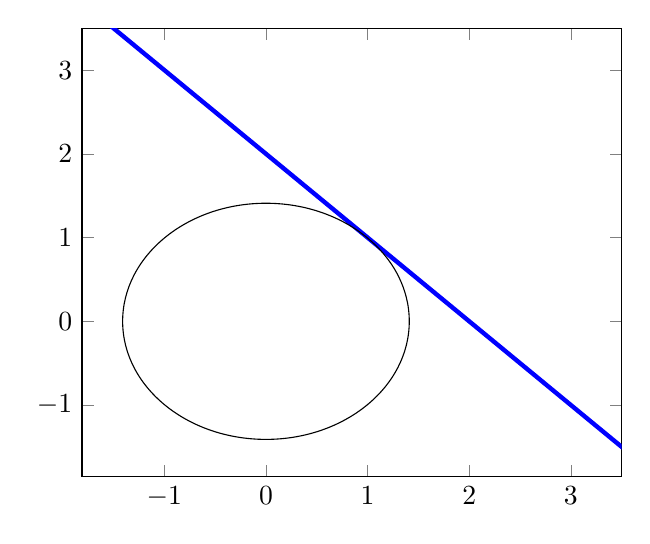
\begin{tikzpicture}
\begin{axis}[xmax=3.5,ymax=3.5, samples=50]
  \addplot[blue, ultra thick] (x,2-x);
  \draw (axis cs:0,0) circle [red, radius=1.41];
\end{axis}
\end{tikzpicture}
    \caption{aaa}\label{aaaa}
  \end{figure}
  La recta $C_1$ interseca al círculo de forma tangencial en el punto $(1,1)$. De hecho si homogenizamos y buscamos las intersecciones de las curvas proyectivas
  \begin{align*}
     & \tilde C_1\:\ x+y=2z,\\
     & \tilde C_2\:\ x^2+y^2=2z^2,
  \end{align*}
  entonces despejamos $z=\frac{x+y}{2}$. Lo que nos lleva a $x^2+y^2=2\left(\frac{x+y}{2}\right)^2$. Despejando vale que $(X-Y)^2=0$ y no podría ocurrir que $X,Y$ son ambos cero y $X=Y$. Esto nos lleva al punto $[X,X,X]=[1,1,1]\in\tilde C_1\cap\tilde C_2$ y este punto corresponde al punto afín que ya habíamos encontrado.\par
  Nosotros esperábamos dos puntos de intersección, pero no hay manera ni siquiera pasando por los complejos. Sólo obtenemos un punto de intersección y esto ocurre porque la recta interseca de manera tangencial. Este problema es el análogo al de una variable, recuerde que el teorema fundamental del álgebra garantiza la existencia cierto número de raíces para los polinomios. Lo que no hemos mencionado es la \emph{multiplicidad} de la raíz. En este caso vemos que la misma ecuación $(X-Y)^2=0$ nos dice que la raíz tiene multiplicidad dos.\par
  En conclusión sólo encontramos un punto de intersección, incluso después de haber buscado posibles puntos en el infinito. Esto es porque $[1,1,1]$ se debe contar con multiplicidad dos y corresponde con el hecho de que ambas curvas se intersecan de manera tangencial en este punto. De hecho, se ve reflejado en que al resolver el sistema de ecuaciones obtuvimos la ecuación $(X-Y)^2=0$.
\end{Ex}

Este no es el único caso en que esto puede ocurrir y el siguiente ejemplo lo ilustra.

\begin{Ex}
  Considere ahora la curvas
  \begin{align*}
     & C_1\:\ y=x,\\
     & C_2\:\ y^2=x^3.
  \end{align*}
    \red{aregar figura} Estas curvas se intersecan en dos puntos del plano afín. Al homogenizar obtenemos
    \begin{align*}
     & \tilde C_1\:\ X-Y=0,\\
     & \tilde C_2\:\ X^3-Y^2Z=0,
  \end{align*}
  y resolviendo llegamos a $X^3-X^2Z=0$ y de aquí que $X=0$ ó $X=Y=Z$. Si $X=0$, entonces $Y=0$ y así $Z$ queda libre lo que nos lleva a los puntos $[1,1,1]$ y $[0,0,1]$. A diferencia del caso anterior, no hay multiplicidades mayores a uno. Aquí lo que ocurre es que uno de los puntos de intersección es un punto que no es suave. Las rectas cuyas direcciones aproximan la identidad tienen dos puntos de intersección con la curva cuspidal, entonces en el límite, el punto singular $[0,0,1]$ tiene multiplicidad dos. \red{agregar figura}
\end{Ex}

\begin{Ex}
  Esta vez consideramos las curvas
  \begin{align*}
     & C_1\:\ x+y+1=0,\\
     & C_2\:\ 2x^2+xy-y^2+4x+y+2=0.
  \end{align*}
  Aquel que esté atento podrá notar que
  $$2x^2+xy-y^2+4x+y+2=(x+y+1)(2x-y+2)$$
  y así $C_1\subseteq C_2$ lo que nos dice que la cantidad de puntos de intersección es infinita. Pero entonces las situaciones así no deben entrar en la consideración de los puntos de intersección de manera tan vaga. En el caso de $\bA^2_\bR$ hay infinitos puntos por lo que debemos especificar lo que buscamos.
\end{Ex}

\begin{Def}
  Sea $C\:\ f(x,y)=0$ una curva con $f\in K[x,y]$. Si factorizamos $f$ como un producto de polinomios irreducibles $f=\prod_{j=1}^{n}p_j$, entonces los \term{componentes} de la curva $C$ son las curvas $C_j\:\ p_j(x,y)=0$. Diremos que $C$ es irreducible cuando tenga un único componente. Es decir, sólo si el polinomio $f$ es irreducible.
\end{Def}

\begin{Ex}
  De las curvas estudiadas en el ejemplo anterior, la curva $C_1$ es irreducible al ser un polinomio lineal y la segunda curva se puede factorizar en dos componentes. Ambas rectas son las componentes irreducibles de esta curva.
\end{Ex}

\begin{Def}
  Diremos que dos curvas afines $C_1, C_2$ no tienen componentes en común si sus componentes irreducibles son distintos.
\end{Def}

Un resultado básico en teoría de curvas que no vamos a demostrar es el siguiente:

\begin{Prop}
  Si $C_1, C_2$ son dos curvas afines sin componentes en común, entonces $C_1\cap C_2$ es un conjunto finito.
\end{Prop}

\begin{Rmk}
  De manera análoga al caso afín, se definen componentes de curvas proyectivas y la noción de dos curvas proyectivas sin componentes comunes.
\end{Rmk}

El teorema de Bezout es más general que este resultado. Con lo que hemos visto hasta ahora, lo podemos enunciar.\red{bajé a agarrar agua}\par
Por ahora mencionamos las siguientes propiedades:
\begin{enumerate}
  \item Si $P\not\in C_1\cap C_2$, entonces $I(C_1\cap C_2,P)=0$.
  \item Si $P\in C_1\cap C_2$ y $P$ es un punto no singular de $C_1$ y $C_2$, y si adicionalmente $C_1$ y $C_2$ tienen direcciones tangenciales diferentes en $P$, entonces $I(C_1\cap C_2,P)=1$. En este caso, se dice que $C_1$ y $C_2$ se intersecan en $P$ de manera transversal.
  \item Si $P\in C_1\cap C_2$ y $C_1$ y $C_2$ no se intersecan transversalmente, entonces $I(C_1\cap C_2,P)\geq 2$.
\end{enumerate}

\begin{Th}[Bezout]
  Sean $C_1,C_2\subseteq\bP_\bC^2$ sin componentes en común. Entonces vale que
  $$\sum_{P\in C_1\cap C_2}I(C_1\cap C_2,P)=\deg(C_1)\deg(C_2).$$
  En particular si $C_1,C_2$ son suaves y únicamente tienen intersecciones transversales, entonces
  $$|C_1\cap C_2|=\deg(C_1)\deg(C_2)$$
  y en todo momento se tiene la desigualdad $|C_1\cap C_2|\leq\deg(C_1)\deg(C_2)$.
\end{Th}

\section{Día n+2| 20210114}

\subsection{Multiplicidad de la intersección de dos curvas}
Vamos a estudiar algunas propiedades y ejemplos de cálculo de la multiplicidad o índice de intersecciones $I(C_1\cap C_2,P)$. Vamos a comenzar con un teorema que establece la existencia de la multiplicidad de la intersección y nos permite hacer cálculos.\par

Rápidamente para poder simplificar la notación introducimos los conceptos de variedad.

\begin{Def}
  La \term{variedad afín} de $f$ es el conjunto de ceros de $f$ dentro del espacio afín $\bA^2$. Denotamos
  $$V(f)=\set{x\in\bA^2\:\ f(x)=0}$$
  y análogamente la \term{variedad proyectiva} de $F$ es su conjunto de ceros dentro del espacio proyectivo. Este conjunto es
  $$V(F)=\set{X\in\bP^2\:\ F(X)=0}.$$
\end{Def}
\begin{Th}
  Considere $V(f),V(g)$ dos curvas afines en $\bA_\bC^2$ y $P\in\bA_\bC^2$ dado. Entonces existe un número $I(V(f)\cap V(g),P)$ definido de manera única tal que las siguientes propiedades se satisfacen:
  \begin{enumerate}
    \item $I(V(f)\cap V(g),P)\in\bZ_{\geq 0}$, a menos que $P$ esté en un componente común de $V(f),V(g)$ y en ese caso $I(V(f)\cap V(g),P)=\infty$.
    \item $I(V(f)\cap V(g),P)=0$ si y sólo si $P\not\in V(f)\cap V(g)$.
    \item Dos rectas distintas se intersecan con multiplicidad uno en su punto de intersección.
    \item $I(V(f)\cap V(g),P)=I(V(g)\cap V(f),P)$.
    \item Si $f=\prod p_i^{\al_i}$ y $g=\prod q_i^{\bt_i}$, entonces
    $$I(V(f)\cap V(g),P)=\sum_{i,j}\al_i\bt_jI(V(p_i)\cap V(q_j),P).$$
    \item $I(V(f)\cap V(g),P)=I(V(f)\cap V(g+hf),P)$ para $h\in\bC[x,y]$.
 \end{enumerate}
\end{Th}

\begin{Def}
  El número $I(V(f)\cap V(g),P)$ se llama \term{multiplicidad de la intersección} de $V(f)$ y $V(g)$ en $P$.
\end{Def}

\begin{Ex}
  \begin{enumerate}
    \item $x^2$ con $y$
    \item círculo con recta
    \item cuspidal con identidad
  \end{enumerate}
\end{Ex}

\begin{Def}
  Sea $f$ un polinomio con coeficientes en $\bC$ y $P\in V(f)$. La \term{multiplicidad} de $f$ en $P$
\end{Def}

\chapter{Análisis de Fourier}

\section{Día k| 20210203}
\subsection{La tranformada de Fourier}

Trabajaremos en $\bR^d$ con $m$ la medida de Lebesgue, las funciones a considerar son $f\:\bR^d\to\bC$ y suponemos que son Borel medibles. De aquí tenemos el espacio
$$L^p(\bR^d)=\Set{f\:\bR^d\to\bC\ \text{medible},\ \int\limits_{\bR^d}|f(x)|^p\dd x<\infty}$$
para $p\in[1,\infty[$. En el caso cuando $p=\infty$ tenemos que $\nm{f}_\infty=\esssup(f)$ como el $\inf_{C>0}\set{m(|f|\geq C)=0}$ y definimos $L^\infty$ de manera análoga a $L^p$ como $\set{\nm{f}_\infty>\infty}$. Trabajamos también con el espacio $C_0$... 
\red{estaba cambiando el word wrap}\par
Así, $f$ es integrable cuando $f_r$ y $f_i$ lo sean.\par 
Si $z\in\bC,\ z=x+iy$ definimos el módulo complejo como $|z|=\sqrt{x^2+y^2}$. El módulo complejo cumple algunas propiedades tales como la desigualdad triangular para integrales $\left|\int f\dd x\right|\leq\int|f|\dd x$. Recordemos la identidad de Euler, si $x\in\bR$ entonces $e^{ix}=\cos(x)+i\sin(x)$ y este número tiene módulo 1.

\begin{Def}
  Sea $f\in L^1(\bR^d)$, definimos su \term{transformada de Fourier} como
  $$\cF(f)(\xi)=\hat f(\xi)=\int\limits_{\bR^d}f(x)e^{-2\pi i\braket{x}{\xi}}\dd x,\ \xi\in\bR^d.$$
  Note que $|\hat{f}(\xi)|\leq \nm{f}_1$.
\end{Def}

\begin{Th}
  El mapeo $f\mapsto\hat f$ es una aplicación continua entre $L^1$ y $L^\infty$.  Vale que $\nm{\hat f}_\infty\leq\nm{f}_1$. Además si $f\in L^1$ entonces $\hat f$ es una función uniformemente continua.
\end{Th}

\begin{ptcbp}
  Note que inmediatamente de la definición tenemos $|\hat{f}(\xi)|\leq\nm{f}_1$ para $\xi\in\bR^d$ lo que implica $\nm{\hat{f}}_\infty\leq\nm{f}_1$.\par
  Por otro lado considere la cantidad
  \begin{align*}
    |\hat{f}(\xi+h)-\hat{f}(\xi)|=\left|\int f(x)e^{-2\pi i\braket{x}{\xi+h}}\dd x-\int f(x)e^{-2\pi i\braket{x}{\xi}}\dd x\right|\\
  \leq \int|f(x)||e^{-2\pi i\braket{x}{\xi}}||e^{-2\pi i\braket{x}{\xi}}-1|\dd x\\
  =\int|f(x)||e^{-2\pi i\braket{x}{\xi}}-1|\dd x.
  \end{align*}
  La cantidad $|e^{-2\pi i\braket{x}{\xi}}-1|$ tiende a cero conforme $h\to 0$ por lo que aplicando el teorema de convergencia dominada tenemos que $|\hat{f}(\xi+h)-\hat{f}(\xi)|\to 0$ cuando $h\to 0$ independiente de $\xi$. 
\end{ptcbp}

\begin{Lem}[Riemann-Lebesgue]\label{Lem:RiemannLebesgueLemma}
  Si $f\in L^1$, entonces $\hat{f}(\xi)\to 0$ cuando $\nm{\xi}\to\infty$. Es decir, $\hat{f}\in C_0$.
\end{Lem}

\begin{ptcbp}
  Sea $R=\bigtimes_{i\in[d]}[a_i,b_i]\subseteq\bR^d$ un rectángulo en $\bR^d$. Si $f=\ind_R$ entonces tenemos que $f=\prod_{i\in[d]}\ind_{[a_i,b_i]}$.\red{aaaa me perdí}\par
  Vale entonces 
  $$\hat{\ind}_{[a,b]}(\xi)=\int\limits_a^be^{-2\pi ix\xi}\dd x=\int\limits_a^b(\cos(-2\pi x\xi)+i\sin(-2\pi x\xi))\dd x.$$
  Esta cantidad resulta ser $\frac{-1}{2\pi i\xi}(e^{-2\pi ib\xi}-e^{-2\pi ia\xi})$ que tiende a cero cuando $|\xi|\to 0$. Así $\hat{\ind}_R(\xi)\to 0$ cuando $\nm{\xi}\to\infty$.\par
  Para $f\in L^1$ en general, aproximamos con funciones simples cuyas indicadoras son sobre rectángulos.
\end{ptcbp}

Recuerde que la convolución de funciones en $L^1$ es
$$f\ast g(x)=\int f(x-y)g(y)\dd y.$$
La convolución es cerrada en $L^1$, es asociativa y conmutativa.

\begin{Th}
  Tome $f\in L^p, g\in L^1$ para $p\in [1,\infty]$. Entonces $f\ast g\in L^p$ y $\nm{f\ast g}_p\leq\nm{f}_p\nm{g}_1$.
\end{Th}

De este resultado extraemos que la convolución hereda las propiedades más bonitas de sus operandos. 

\begin{ptcbp}
  Por Minkowski tenemos 
  $$\left(\right)$$
  \red{finish}
\end{ptcbp}

\begin{Prop}\label{prop:PropiedadesTransformada}
  Para $f,g\in L^1$ vale que:
  \begin{enumerate}
    \item $\cF(f\ast g)=\cF(f)\cF(g)$.
    \item $\cF(\tau_h f)(\xi)=e^{-2\pi i\braket{h}{\xi}}\cF(f)(\xi)$. Es decir, traslación se convierte en modulación.
    \item Si $A\in O(d)$, el grupo ortogonal en $d$ dimensiones, entonces
    $$\cF(f(A\.))(\xi)=\cF(f(A\xi)).$$
    \item Si $f_\la(x)=\frac{1}{\la^d}f\left(\frac{x}{\la}\right)$ entonces $\cF(f_\la)(\xi)=\cF(f)(\la\xi)$.
    \item $\cF\left(\pdv{f}{x_j}\right)(\xi)=2\pi i\xi_j\cF(f)(\xi)$, cuando $f_j\in L^1$. Y para el otro lado, $\cF(-2\pi ix_j f)(\xi)=\pdv{\xi_j}\cF(f)(\xi)$ cuando $x_jf\in L^1$.
  \end{enumerate}
\end{Prop}

\begin{ptcbp}
  Primero, la transformada de la convolución es 
  $$\int\limits_{\bR^d}(f\ast g)(x)e^{-2\pi i\braket{x}{\xi}}\dd x=\int\limits_{\bR^d}\left(\int\limits_{\bR^d}f(x-y)g(y)\dd y\right)e^{-2\pi i\braket{x}{\xi}}\dd x.$$
  Como $x=x-y+y$ separamos la exponencial por linealidad del producto escalar en $e^{-2\pi i\braket{x}{\xi}}=e^{-2\pi i\braket{x-y}{\xi}}e^{-2\pi i\braket{y}{\xi}}$. 
  Ahora, separamos las integrales en 
  $$\left(\int\limits_{\bR^d}f(x-y)e^{-2\pi i\braket{x-y}{\xi}}\dd x\right)\left(\int\limits_{\bR^d}g(y)e^{-2\pi i\braket{y}{\xi}}\dd y\right)=\cF(f)\cF(g).$$
  Para el segundo inciso, la acción del operador de traslación sobre $f$ es $f(x)\mapsto f(x-h)$, entonces tenemos que
  $$\cF(\tau_h f)(\xi)=\int\limits_{\bR^d}f(x-h)e^{-2\pi i\braket{x}{\xi}}\dd x.$$
  Aplicando el cambio de variables $x\mapsto x+h$ llegamos a 
  $$\int\limits_{\bR^d}f(x)e^{-2\pi i\braket{x+h}{\xi}}\dd x=e^{-2\pi i\braket{h}{\xi}}\int\limits_{\bR^d}f(x)e^{-2\pi i\braket{x}{\xi}}\dd x=e^{-2\pi i\braket{h}{\xi}}\cF(f)(\xi).$$
  Tomemos $A\in O(d)$, entonces 
  $$\cF(f(Ax))(\xi)=\int\limits_{\bR^d}f(Ax)e^{-2\pi i\braket{x}{\xi}}\dd x.$$
  Mapeamos $x$ a $A^{-1}x$ que coincide con $A^\sT x$ y como $A$ es ortogonal, entonces $|\det A|=1$. Así la transformada Es
  $$\int\limits_{\bR^d}f(x)e^{-2\pi i\braket{A^Tx}{\xi}}\dd x=\int\limits_{\bR^d}f(x)e^{-2\pi i\braket{x}{A\xi}}\dd x=\cF(f)(A\xi).$$
  Tomamos ahora la transformada de la dilatación y vemos que 
  $$\cF(f_\la)(\xi)=\int\limits_{\bR^d}\frac{1}{\la^d}f\left(\frac{x}{\la}\right)e^{-2\pi i\braket{A^Tx}{\xi}}\dd x.$$
  Luego tomando el cambio de variables $x\mapsto \la x$, el término $\la^{-d}$ está listo para cancelar al determinante y así resulta en 
  $$\int\limits_{\bR^d}f\left(x\right)e^{-2\pi i\braket{\la x}{\xi}}\dd x=\int\limits_{\bR^d}f\left(x\right)e^{-2\pi i\braket{x}{\la\xi}}\dd x\cF(f)(\la\xi).$$
  %Para ver el apartado de las derivadas analizamos primero 
  %$$\cF\left(\pdv{f}{x_j}\right)(\xi)=\int\limits_{\bR^d}f_j\left(x\right)e^{-2\pi i\braket{\la x}{\xi}}\dd x$$
  \red{Ver \cite{Zygmund} pgs 385-386 o usar integración por partes} 
\end{ptcbp}
Note que a partir del último punto, podemos iterar con derivadas de orden superior cuando todo esté bien definido. Vale por ejemplo que
$$\cF\left(\pdv[2]{f}{x_j}{x_k}\right)(\xi)=(2\pi i\xi_j)(2\pi i\xi_k)\cF(f)(\xi).$$
Naturalmente nos preguntamos, 
\begin{significant}
  ¿Se puede recuperar $f$ por medio de $\cF(f)$?
\end{significant}
Cuando se trabaja con series de Fourier, se puede recuperar $f$ por medio de sus coeficientes de Fourier. Lo esperado es que $f(x)=\int\hat{f}(\xi)e^{2\pi i\braket{x}{\xi}}\dd\xi$. Pero $\hat{f}$ no necesariamente es integrable.

\subsection{La clase de Schwartz}

Indistintamente hablaremos de la derivada parcial de $f$ respecto a $x_j$ como $\del_j f$ o $D_j f$. La $m$-ésima derivada será en su lugar $\del_j^m f$ o $D_j^m f$. Introducimos brevemente la notación multi-índice, si $\al\in\bN^d$ entonces
$$D^\al f=D_1^{\al_1}\.\dots\.D_d^{\al_d}f.$$
Por ejemplo $D^{(3,1,4)}f=\frac{\del^8f}{\del x_1^3\del x_2\del x_3^4}$. También tenemos $\al!=\prod\al_j!$ y $x^\al=\prod x_j^{\al_j}$.

\begin{Def}
  Una función $f$ está en la \term{clase de Schwartz} $\cS(\bR^d)$ si es infinitamente diferenciable y todas sus derivadas decrecen rápidamente a infinito. Es decir para $\al,\bt$ multi-índices vale
  $$\sup_{\bR^d}|x^\al D^\bt f(x)|=\rho_{\al,\bt}(f)<\infty.$$
\end{Def}

Inmediatamente de la definición $\Coo_c\subseteq\cS$, también $\rho_{\al,\bt}$ es una seminorma lo que nos puede llevar a una topología. El conjunto $\set{\rho_{\al,\bt}}$ es una familia contable. Entonces $(f_n)\to 0$ en $\cS$ cuando $\rho_{\al,\bt}(f_n)\to 0$ para $\al,\bt$ son cualquier multi-índice. Podemos ver que $\cS$ es un espacio de Fréchet, la métrica que se puede definir es
$$d(f,g)=\sum_{j\in\bN}\frac{\rho_j(f-g)}{2^j(1+\rho_j(f-g))},$$
donde $(\rho_j)$ es una enumeración de las seminormas.

\begin{Th}
  Ocurre que $\cS$ es denso en $L^p$ para $p\in[1,\infty[$.
\end{Th}

Note que si valiese que $\cS\subseteq L^p$ entonces, como $\Coo_c\subseteq\cS$ y $\Coo_c$ es denso ya entonces estaríamos listos. Basta probar que el espacio de Schwartz está en $L^p$.

\begin{ptcbp}
  Tome $f\in\cS$, entonces 
  \begin{align*}
    \int|f|^p\dd x&=\int(1+|x|^{d+1})\frac{|f|}{1+|x|^{d+1}}\\
    &\leq \int\frac{c(|f|+\sum_{j\in[d]}|x_j|^{2d+2}|f|)^p}{(1+|x|^{d+1})^p}\dd x\\
    &\leq \int\frac{c(\rho_{0,0}f+\sum_{j\in[d]}\rho_{(2d+2)e_j,0}f)^p}{(1+|x|^{d+1})^p}\dd x\\
    &\leq c_2\int\frac{\dd x}{(1+|x|^{d+1})^p}<\infty
  \end{align*} 
  \red{no terminé}
\end{ptcbp}

En particular, el espacio de Schwartz está contenido en $L^1$ y por tanto podemos definir la transformada de Fourier en $\cS$.

\begin{Th}
  El mapeo $f\mapsto\hat f$ es continuo sobre $\cS$ y cumple:
  \begin{enumerate}
    \item $\int f\hat g=\int\hat fg$.
    \item Vale la fórmula de inversión
     $$f(x)=\int\hat f(\xi)e^{2\pi i\braket{x}{\xi}}\dd\xi.$$
  \end{enumerate}
\end{Th}

Precisamos un par de lemas antes de probar este resultado. Note que la fórmula de inversión tiene \emph{casi} las misma forma que la fórmula que la transformada ordinaria. En cierto sentido $f(x)=\hat{\hat f}(-x)$.

\begin{Lem}
Si $f(x)=e^{-\pi\nm{x}^2}$, entonces $\hat{f}=f$. 
\end{Lem}

\begin{ptcbp}
  \red{me salté la prueba, DO}
\end{ptcbp}

Ahora podemos probar el teorema de la fórmula de inversión.

\begin{ptcbp}
  Tenemos que para $f\in\cS$ y $\al,\bt$ multi-índices vale que 
  \begin{align*}
    \xi^\al D^{\bt}\hat{f}(\xi)&=(\prod\xi_j^{\al_j})(D_{\xi_1}^{\bt_1}\dots D_{\xi_d}^{\bt_d})\hat{f}(\xi)\\
    &=C(\cF((D_{\xi_1}^{\bt_1}\dots D_{\xi_d}^{\bt_d})(\prod_{j\in[d]}x_j^{\bt_j})))\dots
  \end{align*}
  $D^\al(x^\bt f)$ es una suma de monomios por derivadas de $f$.
\end{ptcbp}

\section{Día k+1| 20210204}

\subsection{La transformada de Fourier en $L^2$}
\red{anotación sobre el conjugado y extensión a L2.}\par

En $L^2$ por tanto existe una extensión de la transformada de Fourier. Los límites en el enunciado del teorema son consecuencia de la continuidad de la transformada pues lo que tenemos es que $f\ind(B(0,R))\to f$ y $\hat f\ind(B(0,R))\to \hat f$ donde ambas convergen en $L^2$. Esto se conoce como extender el operador por densidad y más adelante veremos cómo extender esto a $L^p$ para $p>2$.

Vimos que en $L^1$ no necesariamente hay inversa de la transformada porque esta no necesariamente es integrable. Tomemos $f\in L^1(\bR^d)$, esperamos que $f(x)=\int\limits_{\bR^d}\hat{f}(\xi)e^{2\pi i\braket{x}{\xi}}\dd\xi$ en algún sentido de convergencia. Sin embargo no estamos asumiendo que $\hat{f}$ es integrable, puede que dicha integral ni siquiera tenga sentido. Aún siendo $f$ la indicadora de un intervalo, la integral en cuestión no existe.

\begin{Ex}
  Si $f=\ind([-a,a])$, entonces $\hat{f}(\xi)=\frac{\sin(\pi a\xi)}{\pi a\xi}$ y esta función no es integrable en el sentido de Lebesgue.
\end{Ex}

Dado esto, necesitamos aplicar métodos de sumabilidad. 

%\subsection{Sumabilidad de Abel}
\begin{Def}
  Sea $\eps>0$, definimos la \term{media de Abel} de $f$ como 
  $$A_\eps f=\int\limits_{\bR^d}$$
\end{Def}

\begin{Def}
  Si definimos $G_\eps f=\int f(x)e^{-\eps\nm{x}^2}\dd x$ para $\eps>0$, entonces decimos que $\int f$ es \term{Gauss sumable} a $\l$ si $\lim_{\eps\to 0}G_\eps f=\l$.
\end{Def}

Ambos promedios se pueden escribir de la forma
$$M_{\eps,\Phi}f=M_\eps f=\int\limits_{\bR^d}\Phi(\eps x)f(x)\dd x$$
con $\Phi\in\cC_0$ y $\Phi(0)=1$.

Entonces la idea es modificar un poco las cosas para obtener cierta convergencia. Para lo que queremos hacer, necesitamos las transformadas de Fourier de $e^{-\eps\nm{x}^2}$ y $e^{-\eps\nm{x}}$. Sabemos que $\cF(e^{-\pi\nm{x}^2})(\xi)=e^{-\pi\nm{\xi}^2}$ por lo que para tener la de $\eps$ basta con hacer una dilatación. Si llamamos $g(x)=e^{-\pi\nm{x}^2}$, entonces $e^{-\eps\nm{x}^2}=g\left(\sqrt{\frac{\eps}{\pi}}x\right)$ y como $\cF(\la^{-d}h(\la^{-1}x))=\hat{h}(\la\xi)$, entonces tendremos que 
$$\cF(e^{-\eps\nm{x}^2})(\xi)=\red{calc}.$$

\begin{Th}
  En general, si $a>0$, tenemos que 
  $$\int\limits_{\bR^d}e^{-\pi a\nm{x}^2}e^{-2\pi i\braket{x}{\xi}}\dd x=a^{-\frac{d}{2}}e^{-\frac{\pi}{a}\nm{\xi}^2}.$$
  También vale que 
  $$\int\limits_{\bR^d}e^{-2\pi a\nm{x}}e^{-2\pi i\braket{x}{\xi}}\dd x=c(d)\frac{a}{(a^2+\nm{\xi}^2)^{\frac{d+1}{2}}}$$
  con $c(d)=\frac{\Ga\left(\frac{d+1}{2}\right)}{\pi^{\frac{d+1}{2}}}$.
\end{Th}

\begin{ptcbp}
  \red{Ejercicio}
\end{ptcbp}

Para simplificarnos los cálculos, llamemos $W=W(\xi,a)=\cF(e^{-4\pi^2a\nm{\.}^2})$ y $P=P(\xi,a)=\cF(e^{-2\pi a\nm{\.}})$. A $W$ lo conocemos como el \term{núcleo de Gauss-Weierstrass} y $P$ como el \term{núcleo de Poisson}.\par 
Así, queremos probar que las medias de Abel y Gauss de $\int\hat{f}\exp(2\pi i\braket{x}{\xi})\dd\xi$ convergen a $f$ en norma y casi por doquier. Esto nos diría que 
$$f(x)=\int\limits_{\bR^d}\hat{f}(\xi)e^{2\pi i\braket{x}{\xi}}w(\xi)\dd\xi$$
lo que nos permite recuperar $f$ por medio de su transformada.\par 
Tomemos $\Phi\in\cC_0\cap L^1$, con $\Phi(0)=1$. Llame $\vf=\hat\Phi$ y $\vf_\la=\la^{-d}\vf(\la^{-1}x)$ para $\la$ positivo. Con esta notación vale que 
\begin{gather*}
  \Phi(x)=\exp(-4\pi^2\nm{x}^2)\To\vf_\eps=W(algo),\\
  \Phi(x)=\exp(-2\pi\nm{x})\To\vf_\eps=P(\xi,\eps).
\end{gather*}
 
\begin{Th}\label{thm:tmaPendPara0208}
  Si $f,\Phi\in L^1(\bR^d)$ y $\vf=\hat\Phi$, entonces 
  $$\int\hat{f}(\xi) e^{2\pi i\braket{x}{\xi}}\Phi(\eps\xi)\dd\xi=\int f(x)\vf_\eps(x-\xi)\dd x,\ \eps>0.$$
  En particular, $\int\hat{f}(\xi)e^{2\pi i\braket{x}{\xi}}e^{-2\pi \eps\nm{\xi}}\dd\xi=\int f(x)P(x-\xi,\eps)\dd x$.
\end{Th}

La prueba del teorema se basa en la fórmula $\int f\hat g=\int\hat fg$ a $f$ y a $\Phi(\eps x)e^{2\pi i\braket{x}{\xi}}$. Resta por notar que los núcleos con los que estamos trabajando, ambos integran a uno. La prueba de estos hechos es un \red{ejercicio}.

\begin{Th}\label{thm:segundoTmaPendPara0208}
  Si $\vf\in L^1$ con $\int\vf=1$ y para $\eps>0$ definimos $\vf_\eps(x)=\frac{1}{\eps^d}\vf\left(\frac{x}{\eps}\right)$, entonces si $f\in L^p\cup\cC_0$ para $1\leq p<\infty$, vale que 
  $$\nm{f\ast\vf_\eps-f}_p\to 0,\quad \eps\to 0.$$
  Por otro lado, cuando $f$ sólo está en $\cC_0$, la convergencia es en norma de $L^\infty$. En particular $\int f(\xi)P(x-\xi,\eps)\dd\xi$ y $\int f(\xi)W(x-\xi,\eps)\dd\xi$ convergen a $f$ en $L^p$ cuando $\eps\to 0$.
\end{Th}

\section{Día k+2| 20210208}

\subsection{Un breve resumen}

Teníamos una función $\Phi\in L^1$, con $\hat\Phi=\vf$ y $\vf_\eps(x)=\eps^{-d}\vf(\eps^{-1}x)$. El efecto del $\eps$ en el argumento es dilatar un poco el dominio mientras que el exterior dilata el rango, más su uso es normalizar el determinante del Jacobiano en $\bR^d$.\par 
En el contexto del teorema \ref{thm:tmaPendPara0208}, la integral 
$$\int\hat{f}(\xi) e^{2\pi i\braket{x}{\xi}}\Phi(\eps\xi)\dd\xi$$
se conoce como la $\Phi$-media ó $\Phi$-promedio de $\int\hat{f}(\xi) e^{2\pi i\braket{x}{\xi}}\dd\xi$. Lo que quisiéramos es que el término $f\ast\vf_\eps$, al que la $\Phi$-media es igual, sea convergente a $f$ en algún sentido. Porque así tendremos que las medias de la integral convergen lo que nos dará convergencia de la transformada en algún sentido.

\begin{Ex}
  Nosotros teníamos varios ejemplos de estas funciones.
  \begin{gather*}
    \Phi(x)=e^{-2\pi\nm{x}},\ \vf(\xi)=\frac{c_d}{(1+\nm{\xi}^2)^{\frac{d+1}{2}}},\ \Phi(\eps x)=e^{-2\pi\eps\nm{x}},\ \vf_\eps(\xi)=\frac{\eps c_d}{(\eps^2+\nm{\xi}^2)^{\frac{d+1}{2}}},\\
    \Phi^g(x)=e^{-\pi\nm{x}^2},\ \vf^g(\xi)=e^{-\pi\nm{\xi}^2},\ \Phi^g(\eps x)=e^{-\pi\eps^2\nm{x}^2},\ \vf^g_\eps(\xi)=\eps^{-d}e^{-\pi\eps^{-2}\nm{\xi}^2}.
  \end{gather*}
  A la función $P(\xi,\eps)=\vf_\eps(\xi)$, se le conoce como el \term{núcleo de Poisson} y es la transformada de Fourier de $\Phi(\eps x)$. Mientras que $$W(\xi,\eps)=(4\pi\eps)^{-\frac d2}e^{-\frac{\nm{\xi}^2}{4\eps}}=\vf_{2\sqrt{\pi\eps}}^g(\xi)$$
  es una dilatación de $\vf_g$ y la transformada de $\Phi^g(2\sqrt{\pi\eps}x)=e^{-4\pi^2\eps\nm{x}^2}$. A esta función se le conoce como el \term{núcleo de Gauss-Weierstrass}.
\end{Ex}

Con estos dos núcleos podemos aplicar el teorema \ref{thm:tmaPendPara0208}. Nada más recordamos un lema antes de proseguir. 

\begin{Lem}
  Vale que $\int W(\xi,\eps)\dd\xi=\int P(\xi,\eps)\dd\xi=1$ para $\eps>0$.
\end{Lem}

La integral del núcleo de Poisson requiere de cambios a coordenadas polares mientras que el de Poisson sí requiere integración compleja o técnicas que veremos más adelante. Probamos ahora el teorema \ref{thm:segundoTmaPendPara0208}.

%%IMportante https://tex.stackexchange.com/questions/6195
\begin{ptcbp}
  Lo primero es notar que 
  $$\int\vf_\eps(x)\dd x=\int\frac{1}{\eps^d}\vf\left(\frac{x}{\eps}\right)\dd x\stackrel{y=\frac{x}{\eps}}{=}\int\vf(y)\dd y=1.$$
  Y con esta observación vemos que 
  $$f\ast\vf_\eps-f=\int f(x-y)\vf_\eps(y)\dd y-f(x)\int\vf_\eps(y)\dd y=\int(f(x-y)-f(x))\vf_\eps(y)\dd y,$$
  donde buscamos estimar la norma $L^p$ de la última cantidad.\par 
  Estamos ante una situación favorable pues $\vf_\eps$ está controlado ya que tiene integral 1, y como $f$ es ``bien portada'', la diferencia debería también tener un comportamiento razonable. La norma $L^p$ buscada es 
  \begin{align*}
    \nm{f\ast\vf_\eps-f}_p&=\left(\int\left|\int(f(x-y)-f(x))\vf_\eps(y)\dd y\right|^p\dd x\right)^{\frac 1p}\\
    \colorbox{celesteUCR}{(\text{Minkowski})}&\leq \int\left(\int(|f(x-y)-f(x)||\vf_\eps(y)|)^p\dd x\right)^{\frac{1}{p}}\dd y\\
    &=\int\left(\int |f(x-y)-f(x)|^p\dd x\right)^{\frac{1}{p}}|\vf_\eps(y)|\dd y\\
    \textcolor{celesteUCR}{\left(\substack{ \eps^{-1}y\mapsto y\\
    \dd y\mapsto \eps^{-d}\dd y}\right)}&=\int\left(\int |f(x-\eps y)-f(x)|^p\dd x\right)^{\frac{1}{p}}|\vf(y)|\dd y.
  \end{align*}
  Esta última expresión ya se ve mejor pues $\vf\in L^1$ y la otra integral se puede acotar por $2\nm{f}_p$. Es decir acotamos por un múltiplo de una función integrable. Si podemos ver que esto converge a cero, podemos aplicar el teorema de convergencia dominada.\par 
  Si $f$ es continua y de soporte compacto, entonces es fácil ver que $\int |f(x-\eps y)-f(x)|^p\dd x$ tiende a cero. Al integrar sobre un compacto de medida finita obtenemos la cota de $\eps$ por la medida del soporte y por continuidad la diferencia tiende a cero. Luego por densidad\footnote{Una prueba de este hecho genera una función explícita a partir del lema de Urysohn.} en $L^p$, este procedimiento vale para $f\in L^p$.\par 
  Concluimos, por el teorema de convergencia dominada, que $\nm{f\ast\vf_\eps-f}_p\to 0$ cuando $\eps\to 0$.
\end{ptcbp}

Pegamos esto con el teorema \ref{thm:tmaPendPara0208} para ver que la integral $\int\limits_{\bR^d}\hat{f}(\xi)e^{2\pi i\braket{x}{\xi}}w(\xi)\dd\xi$ va a converger a $f(x)$ en norma $L^p$. A manera de corolario entonces tenemos:

\begin{Cor}\label{cor:convLpFTxPhiMean}
Si $f,\Phi\in L^1$, y $\vf=\hat\Phi\in L^1$ con $\int\vf=1$, entonces
$$\int\hat{f}(\xi)e^{2\pi i\braket{x}{\xi}}\Phi(\eps\xi)\dd\xi\xrightarrow[]{L^p}f(x),\ \eps\to 0.$$
\end{Cor}

Entonces con esto vemos que la integral de la transformada inversa no converge por si sola sino que requiere ayuda del $\Phi$-promedio. Al menos podemos recuperar de una forma la función original a partir de la transformada de Fourier.\par 
El caso particular de este resultado es usar los núcleos de Gauss-Weierstrass y Poisson.

\begin{Cor}
  Si $f\in L^1$, entonces vale que:
  \begin{itemize}
    \item $\int\hat{f}(\xi)e^{2\pi i\braket{x}{\xi}}e^{-4\pi^2\eps\nm{\xi}^2}\dd\xi\xrightarrow[]{L^1}f(x)$ cuando $\eps\to 0$.
    \item $\int\hat{f}(\xi)e^{2\pi i\braket{x}{\xi}}e^{-2\pi\eps\nm{\xi}}\dd\xi\xrightarrow[]{L^1}f(x)$ cuando $\eps\to 0$.
  \end{itemize}
\end{Cor}

Hasta ahora hemos visto que la integral de la transformada de Fourier sólo tiene sentido cuando asumimos que $f$ es integrable, la integral que define la transformada inversa también tiene sentido cuando $f$ es integrable. Pero aún cuando tiene sentido no quiere decir que la integral resulte ser $f$. 

\begin{Cor}
  Suponga que ambas $f$ y $\hat{f}$ están en $L^1$, entonces vale
  $$f(x)=\int\hat{f}(\xi)e^{2\pi i\braket{x}{\xi}}\dd\xi$$ %%Discrepancia con signo negativo en exp
  casi por doquier.
\end{Cor}

\begin{ptcbp}
  El corolario anterior garantiza que 
  $$\int\hat{f}(\xi)e^{2\pi i\braket{x}{\xi}}e^{-4\pi^2\eps\nm{\xi}^2}\dd\xi\xrightarrow[]{L^1}f(x)$$
  donde ahora el término $\hat{f}(\xi)e^{2\pi i\braket{x}{\xi}}e^{-4\pi^2\eps\nm{\xi}^2}$ está dominado. La primera exponencial tiene módulo 1 y la otra es una exponencial real con exponente negativo y así, está acotado por 1. Entonces todo está dominado por $\hat{f}$ que está en $L^1$.\par 
  Por convergencia dominada, vale que 
  $$\lim_{\eps\to0}\int\hat{f}(\xi)e^{2\pi i\braket{x}{\xi}}e^{-4\pi^2\eps\nm{\xi}^2}\dd\xi=\int\hat{f}(\xi)e^{2\pi i\braket{x}{\xi}}\dd\xi$$
  en $L^1$ lo que garantiza convergencia casi por doquier.
\end{ptcbp}

Recordemos ahora que cuando $f\in L^1$, su transformada es uniformemente continua y si a su vez la transformada está en $L^1$, lo mismo ocurre para $\int\hat f(\xi)e^{2\pi i\braket{x}{\xi}}\dd \xi$. Eso quiere decir que $f(x)$ es igual casi por doquier a una función uniformemente continua. Para efectos de la medida, $f$ es continua. En cuyo caso, la igualdad $f(x)=\int\hat f(\xi)e^{2\pi i\braket{x}{\xi}}\dd \xi$ pasa de ser casi por doquier a siempre. Si no, se puede modificar en un conjunto de medida cero para que sea continua y la igualdad valga para todo $x$. Sin embargo, estamos asumiendo algo bastante fuerte que es que $\hat{f}\in L^1$ y \emph{eso no siempre es el caso}.\par 
Del resultado anterior se desprende que cuando la transformada es cero, $f$ es cero casi por doquier. También podemos verlo incluso del corolario \ref{cor:convLpFTxPhiMean} anterior, pues $f$ va a ser el límite de cosas que son cero.

\begin{Cor}[Unicidad de la transformada]
  Si $f,g\in L^1$ y $\hat{f}=\hat{g}$, entonces $f=g$ casi por doquier. 
\end{Cor}

\begin{ptcbp}
  Sea $h=f-g$, entonces $\hat{h}=0$. Luego, por el teorema \ref{thm:segundoTmaPendPara0208} vale
  $$\nm{\int\hat{h}(\xi)e^{2\pi i\braket{x}{\xi}}\Phi(\eps\xi)\dd\xi-h(x)}_1\to0$$
  y como los términos de la izquierda son cero, se sigue que $\nm{h}_1\to0$. Concluimos que $h=0$ casi por doquier.
\end{ptcbp}

\subsection{Convergencia puntual}

Hemos hablado de convergencia en norma, pero ahora vamos a hablar de convergencia puntual. Esto porque vamos a eliminar la suposición de que $\hat{f}$ está en $L^1$ y vamos a usar herramientas distintas. Algunas de estas serán el teorema de diferenciación de Lebesgue, la fórmula de coordenadas polares en $\bR^d$ y la desigualdad de Hölder. 

\begin{Th}[Diferenciación de Lebesgue]\label{thm:}
  Si $f\in L^1_\loc$, entonces
  $$\frac{1}{m(B_r(0))}\int\limits_{B_r(0)}(f(x-y)-f(x))\dd y\to 0$$
  conforme $r\to 0$.
\end{Th}
%%Min 55
\section{Día k+3| 20210209}
\section{Día k+4| 20210210}
\section{Día k+5| 20210211}

La vez pasada hemos hablado sobre distribuciones de soporte compacto. Recordemos la definición \red{ref y agregar defn sig en día anterior}

\begin{Def}
  Para $u\in\cD'$, diremos que $\supp(u)$ es la intersección de los cerrados $F$ tales que si $\vf\in\Coo_c$ con $\supp(\vf)\subseteq F^c$, entonces $(\vf,u)=0$. %Vista como par dual
\end{Def}

También vimos que el dual de $\Coo$, el conjunto $\cE'$ de las distribuciones con soporte compacto sólo era un nombre. Queremos ver que en efecto tienen soporte compacto de acuerdo con esta definición. Teníamos también la caracterización

$$u\in\cD'\iff \forall K\ \text{compacto}\ \exists C>0,\ m\in\bN(|(f,u)|\leq C\sum_{|\al|\leq m}\nm{D^\al f}_\infty)$$

para $f\in\Coo_c$ con $\supp(f)\subseteq K$. Y la caracterización de $\cE'$ resulta ser 

$$u\in\cE'\iff \exists C>0,\ m,N\in\bN(|(f,u)|\leq \sum_{|\al|\leq m}\tilde{\rho_{\al,N}(f)})$$

donde $f\in\Coo$ y $\tilde{\rho}_{\al,N}(f)=\sup_{\nm{x}\leq N}|D^\al f(x)|$. Veremos que una distribución que cumple esta condición también cumple tener soporte compacto de acuerdo a lo anterior.

\begin{ptcbp}
  Sea $u\in\cE'$ y $\vf\in\Coo$ tal que $\supp(\vf)\subseteq B_N(0)^c$ que es un cerrado. Entonces \red{no entendí bien} $\supp(D^\al f(x))\subseteq B_{N+1}(0)^c$ lo que dice que $D^\al f(x)=0$ para $x\in\ov B_N(0)$ y así $\sup_{\nm{x}\leq N}|D^\al f(x)|=0$.\par 
  La condición equivalente nos dice que 
  $$|u(f)|=|(f,u)|\leq\sum_{|\al|\leq m}\sup_{\nm{x}\leq N}|D^\al f(x)|=0.$$
  Esto implica que la acción de $u$ sobre $f$ es cero, fuera del cerrado $\ov B_N(0)$ la acción de $u$ es cero y por tanto $\supp(u)\subseteq \ov B_N(0)$. Concluimos que $u$ tiene soporte compacto de acuerdo con la definición nueva.\par 
  Ahora supongamos que $u$ es de soporte compacto de acuerdo a la definición. Debemos probar la propiedad \red{referenciar referenciar}. Sea $\eta\in\Coo$ tal que $\eta=\ind(B_N(0))(1-\ind(B_{N+1}(0)))$ \red{escribir mejor}. Si consideramos $h(1-\eta)$ para $h\in\Coo_c$, entonces $h(1-\eta)$ tiene soporte disjunto con $u$ lo que nos dice que
  $$(h,u)=(h\eta,u)+(h(1-\eta),u)=(h\eta,u).$$
  Si bien para una función $\Coo$ $u$ no puede actuar, por medio de la igualdad descrita podemos definir la acción. Si $f\in\Coo$, entonces $(f,u)=(f\eta, u)$ y así $u$ es un funcional lineal que actúa en $\Coo$. Por la caracterización de las distribuciones en $\cD'$ vale que 
  $$|(f\eta,u)|\leq\sum_{|\al|\leq m}\nm{D^\al(f\eta)}_{\infty},$$
  donde tenemos que nuestro compacto es $K=\ov B_{N+1}(0)$ y $f\eta$ tiene soporte en $K$. Ahora, ¿qué es $D^\al(f\eta)$ en norma $L^\infty$? Esto es 
  $$\sup_{x}|D^\al(f\eta)(x)|=\sup_{\nm{x}\leq N+1}|D^\al(f\eta)(x)|$$
  y esta última cantidad es una suma de productos de derivadas de $f$ con derivadas de $\eta$ de orden menor o igual a $\al$. Las derivadas de $\eta$ está acotadas por lo que dicho supremo está acotado por una suma finita de seminormas $\rho_{\ga,N+1}$ para $|\ga|\leq m$. \red{finish}
\end{ptcbp}

\begin{Ex}
  Si $F=\ov B_\eps(x_0)$ y tenemos $f$ tal que $\supp(f)\subseteq \ov{B}_\eps(x_0)^c$, entonces $(f,\del_{x_0})=f(x_0)=0$. Así el soporte de la delta de Dirac es $\supp(\del_{x_0})\subseteq\ov B_\eps(x_0)$. Pero esto vale para $\eps>0$ y así vemos que $\supp(\del_{x_0})=\set{x_0}$.
\end{Ex}

\begin{Def}
  Diremos que una distribución $u\in\cD'$ coincide con la función $h$ en un abierto $U$ si 
  $$(f,u)=\int f(x)h(x)\dd x,\ f\in\Coo_c(U).$$
\end{Def}

Esto quiere decir que hay distribuciones que \emph{se pueden ver como funciones}. Pero no todas las distribuciones cumplen esto. A este tipo de expresión se le conoce como una transformación integral. Cuando esto ocurre, el soporte de la distribución $u-h$ está contenido en $U^c$. Aquí $u-h=u-L_h=u-\int(\.)h(x)\dd x$. Como en $U$ la diferencia es cero, entonces su soporte está en $U^c$.

\begin{Ex}
  Sean $a,b\in\bR^d$ y $u=|x|^2+\dl_a+\dl_b$, entonces 
  $$(f,u)=\int f(x)|x|^2\dd x+f(a)+f(b).$$
  Si $U$ es un abierto tal que $a,b\not\in U$, entonces $u$ coincide con $|x|^2$ en el abierto $U$.
\end{Ex}

\begin{Th}
  Si $u\in\cS'$ y $\vf\in\cS$, entonces $\vf\ast u\in\Coo$ y además 
  $$(\vf\ast u)(x)=(\tau_x\tilde{\vf},u),\ x\in\bR^d.$$
  También para $\al\in\bN^d$, existen $c_\al,k_\al$ tales que sus derivadas crecen a lo sumo polinomialmente:
  $$|\del^\al(\vf\ast u)(x)|\leq c_\al(1+\nm{x})^{k_\al}.$$
  Y más aún si $\supp(u)$ es compacto, entonces $\vf\ast u$ es de Schwartz.
\end{Th}

\begin{Def}
  $h\ast u$ se define como $(f,h\ast u)=(\tilde{h}\ast f,u)$ con $\tilde{h}(x)=h(-x)$.
\end{Def}

Esta es la definición de convolución con distribución. Al final es pasarle el trabajo a la función. El teorema lo que dice es que la distribución convolución se puede ver como una función. Se hace la identificación con la función respecto a la cual se integra. 

\begin{ptcbp}
  Tomemos $f\in\cS$, por definición 
  $$(f,\vf\ast u)=(\tilde{\vf}\ast f,u)=u\left(\int\tilde\vf(\.-y)f(y)\dd y\right)$$
  y podemos ver ese $\tilde\vf$ como uan traslación. Entonces esto es 
  $$u\left(\int\tau_y\tilde{\vf}(\.)f(y)\dd y\right)=\int u(\tau_y\tilde{\vf})f(y)$$
  que se asemeja a \emph{operar con elementos de la base}. Este paso se justifica porque $u$ es continua y $\int$ converge en $\cS$. Esto se resumen en $L_{u(\tau_{\.}\tilde{\vf})}(f)$ y así $\vf\ast u$ corresponde con $u(\tau_{\.} \tilde{\vf})$.\par 
  Para ver que es suave calculamos su derivada parcial
  \begin{align*}
    (\vf\ast u)(x+he_j)-(\vf\ast u)(x)&=\tau_{-he_j}(\vf\ast u)\dots\\
    & \red{rip}
  \end{align*}
  Entonces $D_j(\vf\ast u)(x)=u(\tau_x(D_j\tilde{\vf}))=D_j\vf\ast u$. El mismo cálculo muestra que $\vf\ast u\in\Coo$ y que $D^\ga(\vf\ast u)=(D^\ga\vf)\ast u$ para $\ga\in\bN^d$. \par 
  \red{calc violento derivada convolución}\par 

A fin de cuentas $\ga$ está acotado en norma, entonces podemos ver que esto está acotado por
$$\sum_{|\bt|\leq k}\sup_y(1+|x|^m+|y|^m)|D^{\al+\bt\tilde{\vf}(y)}|.$$
Tomando supremo en $y$, el término $|y|^m|D^{\al+\bt\tilde{\vf}(y)}|$ está acotado por la seminorma $\rho_{(m,m,\dots,m),\al+\bt}(\tilde{\vf})$ que es una constante. Después de resolver los supremos y demás, esta cantidad termina acotada por $C(1+\nm{x}^m)$. Por lo tanto hay crecimiento polinomial como buscábamos.\par 
\red{finish con Grafakos pag 147}
\end{ptcbp}


\section{Ínterin| Tarea}

\begin{Ej}
  Probar prop 4 (rip, cual era esta)
  \end{Ej}

  Ver \ref{prop:PropiedadesTransformada}
\begin{Ej}
 Muestre que $f\in\cS(\bR^d)$ si y sólo si $f\in\Coo(\bR^d)$ y $|D^\al f(x)|\leq \frac{C(\al,N)}{(1+\nm{x})^N}$ para $\al\in\bN^d$ y $N\in\bN$.
\end{Ej}

\begin{ptcbp}%Folland 237, 2708452 Coto sugirió revisar desigualdades 
  Suponga que $f$ está en la clase de Schwartz, entonces vale que 
  $$\sup_{\bR^d}|x^\al D^\bt f(x)|<\infty$$
  para $\al,\bt\in\bN^d$. Ahora observe que el término \emph{multinomial} cumple que 
  $$|x^\al|\leq C(\al,d)\nm{x}^{\nm{\al}}\leq C(\al,d)\sum_{\nm{\bt}\leq\nm{\al}}|x^\bt|.$$
  La primera desigualdad es quizás la más extraña dada nuestra falta de costumbre a trabajar con términos multinomiales. Es cuestión de escribir lo que está sucediendo y recordar la equivalencia de normas en $\bR^d$. Vea que
  \begin{align*}
    |x^\al|&=|x_1^{\al_1}x_2^{\al_2}\dots x_d^{\al_d}|=|x_1|^{|\al_1|}\dots|x_d|^{|\al_d|}\\
    &\leq (|x_1|+\dots+|x_d|)^{|\al_1|+\dots+|\al_d|}\leq (c(d)\nm{x}_{\l^2})^{\nm{\al}_{\l^1}}\\
    &=C(\al,d)\nm{x}^{\nm{\al}}.
  \end{align*}
  Observe ahora que un término como $(1+\nm{x})^N$ se puede expande con el teorema del binomio como 
  $$(1+\nm{x})^N=\sum_{j=0}^N\binom{N}{j}\nm{x}^j\leq\sum_{j=0}^N\binom{N}{j}C(j,d)\sum_{\nm{\bt}\leq j}|x^\bt|.$$
  Ya con esto podemos ver que 
  \begin{align*}
    (1+\nm{x})^N|D^\al f(x)|&\leq\sum_{j=0}^N\binom{N}{j}C(j,d)\sum_{\nm{\bt}\leq j}|x^\bt D^\al f(x)|\\
    &\leq\sum_{j=0}^N\binom{N}{j}C(j,d)\sum_{\nm{\bt}\leq j}\sup_{\bR^d}|x^\bt D^\al f(x)|=C(\al,d)
  \end{align*}
 
  que es lo que buscábamos.\par 
  Por otro lado, al haber resuelto el la dirección anterior, nos sentimos invitados a tomar $N=\nm\al$. De esta manera note que 
  $$|x^\al|\leq C(\al,d)\nm{x}^{\nm{\al}}\leq C(\al,d)(1+\nm{x})^{\nm{\al}}$$
  donde la última desigualdad se sigue de que el binomio contempla al término $\nm{x}^{\nm{\al}}$ junto con todas las potencias anteriores. De esta manera vea que 
  $$|x^\al D^\bt f(x)|\leq C(\al,d)(1+\nm{x})^{\nm{\al}}|D^\bt f(x)|\leq C(\al,d)\tilde{C}(\bt,\nm{\al}).$$
  Por tanto, tomando supremos sobre $x\in\bR^d$ vemos que $f\in\cS$ según nuestra definición original.
\end{ptcbp}

\begin{Ej}
  Muestre que si $f,g\in\cS(\bR^d)$, entonces $f\ast g\in\cS(\bR^d)$.
\end{Ej}

Previo a mostrar este resultado, precisamos un resultado.

\begin{Lem}
  Bajo la hipótesis del ejercicio, vale que
  $$D^\al(f\ast g)=(D^\al f)\ast g=f\ast D^\al g.$$
\end{Lem}

\begin{ptcbp}
  Veamos que $D^{e_j}(f\ast g)=(D^{e_j}f)\ast g$. Note que 
  $$\frac{1}{h}(f(y+he_j)-f(y))-(\del_jf)(y)\to 0$$
  conforme $h\to 0$. Además para cada $t$, hay una constante que acota la expresión. Integramos respecto a $g(x-y)\dd y$ y vemos que la expresión
  $$\int\limits_{\bR^d}\bonj{\frac{1}{h}(f(y+he_j)-f(y))-(\del_jf)(y)}g(x-y)\dd y$$
  también tiende a cero conforme $h\to 0$ después de aplicar el teorema de convergencia dominada. Dado esto, vale que $D^{e_j}(f\ast g)=(D^{e_j}f)\ast g$ y dado que $\al$ es un multi-índice, el caso general se sigue por iteración de este argumento tanto esta misma entrada como en las demás.
\end{ptcbp}

\begin{ptcbp}%Grafakos 107
  Aprovechamos tanto el lema como el ejercicio anterior. Note que 
  $$\left|\int\limits_{\bR^d}f(x-y)g(y)\dd y\right|\leq C(N)\int\limits_{\bR^d}(1+|x-y|)^{-N}(1+|y|)^{-N-d-1}\dd y,$$
  al estar $f,g$ en la clase de Schwartz según la equivalencia. Ahora como 
  $$(1+|x-y|)^{-N}\leq (1+|y|)^N(1+|x|)^{-N},$$
  podemos reemplazar en la desigualdad previa para ver que
  $$|(f\ast g)(x)|\leq C(N)\int\limits_{\bR^d}(1+|y|)^N(1+|x|)^{-N}(1+|y|)^{-N-d-1}\dd y)=O((1+|x|)^{-N}).$$
  Esto confirma que $f\ast g$ se comporta como $(1+\nm{x})^N$ en infinito. Para ver que sus derivadas también se comportan igual, utilizamos el lema anterior e intercambiamos con uno de los operandos. De esta manera corroboramos que todas las derivadas decaen en infinito y por tanto $f\ast g$ pertenece a la clase de Schwartz.
\end{ptcbp}

\begin{Ej}
  Sea $(f_n)\subseteq\cS$ tal que $f_n\to f$ en $\cS$. Muestre que $\hat{f}_n\to \hat{f}$ y $\check{f}_n\to\check{f}$ en $\cS$.
\end{Ej}

\begin{ptcbp}
  Considerando $\rho_{\al,\bt}(\hat{f}_n-\hat{f})$, buscamos trabajar con el término $|x^\al D^\bt(\hat{f}_n-\hat{f})|$. Entonces cocinamos un poco la derivada aplicando propiedades de la transformada. Vale que 
  $$
    D^\bt(\hat{f}_n-\hat{f})=(-2\pi i)^{\nm{\bt}}\cF(x^\bt(f_n-f))
  $$
  y entonces agregando el $x^\al$ tenemos 
  \begin{gather*}
    (-2\pi i)^{\nm{\bt}}x^\al\cF(x^\bt(f_n-f))=\frac{(-2\pi i)^{\nm{\bt}}}{(2\pi i)^{\nm{\al}}}\cF(D^\al (x^\bt(f_n-f)))\\
    \To|x^\al D^\bt(\hat{f}_n-\hat{f})|\leq \left|\frac{(-2\pi i)^{\nm{\bt}}}{(2\pi i)^{\nm{\al}}}\right||\cF(D^\al (x^\bt(f_n-f)))|\\
    \leq \left|\frac{(-2\pi i)^{\nm{\bt}}}{(2\pi i)^{\nm{\al}}}\right|\nm{D^\al (x^\bt(f_n-f))}_{L^1}.
  \end{gather*}
  Como la multiplicación por polinomios y las derivadas son aplicaciones cerradas en $\cS$, son continuas por el teorema del gráfico cerrado. Concluimos que cuando $f_n-f\to 0$, entonces la última expresión también tiende a cero. Tomando supremos obtenemos lo pedido.\par 
  Con la transformada inversa el trato es similar gracias al teorema de inversión de Fourier en $\cS$. Si $R$ es el operador de reflexión: $f(x)\mapsto f(-x)$, entonces vale $\cF^{-1}=\cF R$ y por tanto podemos usar un argumento similar al anterior.
\end{ptcbp}
%%%%%%%%%%%% Contents end %%%%%%%%%%%%%%%%
\ifx\nextra\undefined
\printindex
\else\fi
\nocite{*}
\bibliographystyle{plain}
\bibliography{bibiTNum}
\end{document} 